\documentclass[12pt, oneside]{article}
%\usepackage[left=2cm,right=2cm,top=2cm,bottom=2cm]{geometry}
\usepackage[utf8]{inputenc}
\usepackage[T1]{fontenc}
\usepackage{lmodern}
\usepackage[left=2.5cm,top=3cm,right=2.5cm,bottom=3cm]{geometry}
%\usepackage[parfill]{parskip}    		% Activate to begin paragraphs with an empty line rather than an indent
\usepackage{graphicx}
%\usepackage{amssymb}
%\usepackage[style=numeric,natbib=true,backend=biber,maxbibnames=9,bibencoding=utf8]{biblatex}
%\addbibresource{"bibliography.bib"}
\usepackage{cite}
\usepackage{courier}
\usepackage{pdflscape}
\usepackage{multirow}
\usepackage{booktabs}
\usepackage{listings}
\usepackage[usenames,dvipsnames]{color}
\usepackage{amsmath}
\usepackage{caption}
\usepackage{subcaption}
\usepackage[colorlinks=false,pdfborder={0 0 0}]{hyperref}
\usepackage{graphicx}

\lstset{basicstyle=\footnotesize\ttfamily,breaklines=true}


\usepackage{booktabs,colortbl}
\usepackage{tabularx}
%\renewcommand{\arraystretch}{1.5}

\usepackage{enumitem}

\newcommand{\red}{\color{red}}
\newcommand{\green}{\color{OliveGreen}}

\usepackage{amsmath}
\usepackage{listings}
\usepackage{color}


\definecolor{dkgreen}{rgb}{0,0.6,0}
\definecolor{gray}{rgb}{0.5,0.5,0.5}
\definecolor{mauve}{rgb}{0.58,0,0.82}

\lstset{frame=tb,
	language=c++,
	aboveskip=3mm,
	belowskip=3mm,
	showstringspaces=false,
	columns=flexible,
	basicstyle={\small\ttfamily},
	numbers=none,
	numberstyle=\tiny\color{gray},
	keywordstyle=\color{blue},
	commentstyle=\color{dkgreen},
	stringstyle=\color{mauve},
	breaklines=true,
	breakatwhitespace=true,
	tabsize=3
}

\title{PMPH project}
\author{Malte Stær Nisssen - tgq958 \\René Løwe Jacobsen - vlx198 \\ Erik John Partridge - xnk343}


\begin{document}
	\maketitle
\section{Project Specifications}
The group project for the course Programming Massively Parallel Hardware is about parallelizing a serial implementation of \texttt{tridag}, contained in the files ProjCoreOrig.cpp, ProjectMain.cpp, ProjHelperFun.cpp, and ProjHelperFun.h. The project consists of three parts: converting to OpenMP parallel, converting to CUDA parallel, and results. We will be comparing the CUDA and OpenMP implementation with the original code. These optimizations and translations were done with the help of the slides from the course, listed in the bibliography. \textsuperscript{\cite{l5slides}\cite{flattening}\cite{projectslides}}
\section{OpenMP}
\subsection{The Idea}
Converting serial loops into parallel loops is as simple as ensuring that there are no loop dependencies. We must check that for every loop we wish to parallelize, that no iteration depends on the results of any other iteration, and that variables which belong to multiple iterations have either the correct scope, so that information does not pass from one iteration to the next, or a separate index for each iteration. After that, we denote the loop ready by adding the appropriate \texttt{\#pragma ...} command, and compiling with the correct options.
\subsection{The Work}
Converting the original code to OpenMP was a straightforward matter, involving only modifying code in ProjCoreOrig.cpp. After ensuring that none of the inner loops would create race conditions, we moved the \texttt{REAL strike} and \texttt{PrivGlobs globs} declarations inside the main loop, and then simply added the line\\
\texttt{\#pragma omp parallel for default(shared) schedule(static) if(outer>8)} right before the same loop declaration. We decided to add the static scheduling line for more than 8 threads, since that was what we were working with. After that, all that was left was to compile with \texttt{g++} using the command line option \texttt{-fopenmp}. The results are displayed in the table on page \pageref{fig:results}.
\subsection{Correctness}
The changes we made were very minor, involving moving 2 variable declarations inwards in scope, and adding the \texttt{\#pragma ...} line. The variable declarations made no difference, since every iteration of the loop resulted in both \texttt{strike} and \texttt{globs} being immediately assigned new values, but moving them allowed for us to parallelize without worrying if the results of one iteration spilled over into another. The \texttt{\#pragma ...} declaration signaled that this loop was able to be run in parallel. We can assure that it was by looking through the code. From the outermost loop, there were no loop dependencies from one iteration to the next: the results were saved in separate \texttt{res[]} indexes, and no result from a previous iteration was used in a later iteration.
\section{CUDA}
\subsection{Preparations}
The code as it stands can be na\"ively converted to CUDA, by replacing the inner loops with the exact same function inside a CUDA kernel. We are going to first implement this, and then continue by optimizing the TRIDAG kernel.
\subsection{Loop Distribution and Array Expansion}
\subsubsection{The Idea}
The first step was to conglomerate every secondary function, which allowed us to hoist the initialization of the globs (global variables) into glob arrays. That is, instead of initializing a temp variable or array for every iteration of a loop, we instead initialize an array one dimension larger, with size equal to the number of iterations of the loop, before the looping code.
\begin{figure}[h]
	\begin{lstlisting}
for (int i = 0; i<max; i++){
	float tmpA = 0.0;
	for (int j = 0; j<max2; j++){
		tmpA += 2*B[j];
		...
	}
	...
}
	\end{lstlisting}
\caption{ \label{fig:nohoist} A code snippet with tmpA initialized for every iteration.}
\end{figure}
\begin{figure}[h]
	\begin{lstlisting}
float tmpA[max] = {0.0, ...};
for (int i = 0; i<max; i++){
	for (int j = 0; j<max2; j++){
		tmpA[i] += 2*B[j];
		...
	}
	...
}
\end{lstlisting}
\caption{ \label{fig:yeshoist} The same code with tmpA hoisted.}
\end{figure}
		
The purpose of this is twofold. First, this allows us to serialize a computation which would otherwise be repeated by every thread. By computing it beforehand, the threads can be spared this extra work. Second, this allows us to easily parallelize the inner loops. Since each iteration of the inner \texttt{j} loop requires access to a single \texttt{tmpA} per iteration of the \texttt{i} loop, we would have to compute it, then pass it on as a variable to each of the threads. In the hoisted version, \texttt{tmpA[]} is copied to device memory, so that the inner loop can just access the appropriate version without much trouble.
\subsubsection{The Work}
The first step for us was to begin preparing the CPU for kernel parallelization. Before distributing the outer loops in ProjCoreOrig.cpp, we began by moving all of the secondary functions (\texttt{updateParams}, \texttt{setPayoff}, \texttt{value}, and \texttt{rollback}) into \texttt{run\_OrigCPU}. This allowed us to easily see the globs and their relations to one another.
		
The work at this step is temporary. The code is objectively de-optimized, since more time is spent on initializing arrays, memory usage is larger, and the code runs slower. The purpose of this is to prepare the code for optimal loop distribution.
		
The \texttt{strike} variable has been removed, being placed instead inside of one of the kernels. The variables which have been hoisted at this step are listed in figure \ref{fig:globs}.

TODO: Something about look distribution

\begin{figure}[h]
\begin{lstlisting}
void   run_OrigCPU(...
{   
	...
	// Generate vector of globs. Initialize grid and operators onces
	// and make default element of vector
	// Hoisted from "value"
	PrivGlobs    globs(numX, numY, numT);
	initGrid(s0, alpha, nu, t, numX, numY, numT, globs);
	initOperator(globs.myX,globs.myDxx);
	initOperator(globs.myY,globs.myDyy);
	vector<PrivGlobs> globArr (outer, globs);
	...
	//Rollback globs
	vector<vector<vector<REAL> > > u(outer,vector<vector<REAL> >(numY, vector<REAL>(numX)));   // [outer][numY][numX]
	vector<vector<vector<REAL> > > v(outer,vector<vector<REAL> >(numX, vector<REAL>(numY)));   // [outer][numX][numY]
	vector<vector<REAL> > a(outer,vector<REAL>(numZ)), b(outer,vector<REAL>(numZ)), c(outer,vector<REAL>(numZ)), y(outer,vector<REAL>(numZ));     // [outer][max(numX,numY)]
	vector<vector<REAL> > yy(outer,vector<REAL>(numZ));  
	// temporary used in tridag  
	// [outer][max(numX,numY)]
	...
\end{lstlisting}
\caption{ \label{fig:globs} Hoisted variables in ProjCoreOrig.cpp. }
\end{figure}
			
The other necessary modifications were to simply update the relevant variable references, for example, changing \texttt{globs.myResult[j][k]} to\\ \texttt{globArr[i].myResult[j][k]}.
\subsubsection{Correctness}
The reason we are allowed to do this is because we are not fundamentally changing anything about the flow of the program. Moving all of the functions together does nothing to program flow, only impeding readability slightly. For the hoisted variables, the extra dimension can be easily compared to a new variable per iteration, and since the variables are moving outwards in scope, nothing vital is changed. There is no danger of loop dependencies, since each iteration still uses their own indexes for these hoisted variables.

TODO: Loop distribution correctness: maps
			
After this work, the program is in a state to distribute the various loops. There is a mild amount of slowdown, since we allocate more memory to some of the variables, and we perform some initial calculations which otherwise performed per loop iteration. This is not a good stopping point, but it is necessary to continue.
\subsection{Kernel Replacement}
\subsubsection{The Idea}
After loop distribution, we began to convert the loops to CUDA kernels. These kernels are copied almost directly from the already existing CPU code. This allowed us to begin using the GPU, and CUDA.
\subsubsection{The Work}
For each of the distributed loops, we na\"ivly translated the code into a CUDA kernel. That is, we attempted to rewrite the functions so that they performed precisely the same task on the GPU as they did on the CPU. Figures \ref{fig:nokernel} and \ref{fig:yeskernel}, show the conversion of the function \texttt{setPayoff} from ProjCoreOrig.cpp into the \texttt{setPayoffKernel} in the file ProjKernels.cu.h. All distributed loops and matching functions were converted.
\begin{figure}[h]
	\begin{lstlisting}
 for(unsigned i = 0; i < outer; ++ i) {
        for(unsigned j=0;j<globArr[i].myX.size();++j)
        {
            for(unsigned k=0;k<globArr[i].myY.size();++k)
            {
                globArr[i].myResult[j][k] = max(globArr[i].myX[j]-0.001*i, (REAL)0.0); // privatized one level in
            }
        }
    }
\end{lstlisting}
\caption{ \label{fig:nokernel} The distributed loop implementation of \texttt{void setPayoff}.}
\end{figure}
\begin{figure}[h]
\begin{lstlisting}
template<const unsigned T>
__global__ void setPayoffKernel(
			const unsigned outer,
			const unsigned numX,
			const unsigned numY,
			REAL* myX,
			REAL* myResult
			)
{
	int i = blockIdx.x*T + threadIdx.x; // outer
	int j = blockIdx.y*T + threadIdx.y; // myX.size
	int k = blockIdx.z*T + threadIdx.z; // myY.size
	if (i < outer && j < numX && k < numY) {
		myResult[i * numX*numY + j * numY + k] = max(myX[i * numX + j]-0.001*i, (REAL)0.0);
	}
}
\end{lstlisting}
\caption{ \label{fig:yeskernel} The equivalent CUDA kernel.}
\end{figure}
					
The next step was to load the appropriate variables to and from memory. Figure \ref{fig:cudamemcopy} shows some of the variables that are now on device memory, to be accessed by the kernels. This is analogous to the \texttt{PrivGlobs} structures from the sequential code.
					
\begin{figure}[h]
\begin{lstlisting}
// Arrays for rollback
REAL* d_a, *d_b, *d_c, *d_y, *d_yy; // [outer][max(numX,numY)]
REAL *d_v, *d_u;
cudaMalloc((void**) &d_a, sizeof(REAL)*outer*numX*numY);
cudaMalloc((void**) &d_b, sizeof(REAL)*outer*numX*numY);
cudaMalloc((void**) &d_c, sizeof(REAL)*outer*numX*numY);
cudaMalloc((void**) &d_y, sizeof(REAL)*outer*numX*numY);
cudaMalloc((void**) &d_yy, sizeof(REAL)*outer*numX*numY);
cudaMalloc((void**) &d_u, sizeof(REAL)*outer*numX*numY);
cudaMalloc((void**) &d_v, sizeof(REAL)*outer*numY*numX);
REAL * timeline = (REAL*) malloc(sizeof(REAL)*numT);
cudaMemcpy(timeline,d_globs.myTimeline,sizeof(REAL)*numT,cudaMemcpyDeviceToHost);
\end{lstlisting}
\caption{ \label{fig:cudamemcopy} Initializing device memory.}
\end{figure}
						
\subsubsection{Correctness}
It is no longer as easy to argue that this is a simple replacement. Transforming the distributed loops into kernels requires that the syntax has to change, and the semantics as well. The example in figure \ref{fig:yeskernel} shows that the loop iteration has been replaced by \texttt{threadIdx}; at a fundamental level, we are moving from sequential loops to parallel threads. The equations are the same, with a slightly more complicated index (\texttt{threadIdx} instead of a simple \texttt{i}), and the variables are now all loaded into GPU memory.
						
The semantics and syntax have both changed from distributed loops to threads but the process is a one-to-one mapping. Every kernel can be directly traced back to a loop, and every loop gave rise to a single kernel. As long as the input and output of the kernels and loops is the same, we have the same program.
						
Although the program has now been distributed to the GPU, the runtime of the entire program took a hit. The problem was, that the first CUDA call of the program also loads the entire CUDA runtime library, which gives a major overhead compared to the actual running time on our datasets. Timing early versions of our code was highly dominated by the CUDA library load time. To combat this, we have added a \texttt{cudaFree(0);} line in the ProjectMain.cu before we start timing.
\subsection{TRIDAG}
The \texttt{tridag} algorithm is a tridiagonal solver, used in systems of continuous differential equations when solved using something known as the Crank-Nicholson finite-difference method. The solution involves large matrix multiplications for the many iterations the finite-differences require, and thus seems like a prime candidate for GPU parallelization. The only problem is that each iteration requires knowledge about the previous iteration, and thus, it is \emph{not} natively fit for parallelization. However, using some variable substitution, we are able to get \texttt{tridag} into a form where we can turn the entire algorithm into a series of scan inclusive operations.
\subsubsection{The Idea}
The original \texttt{tridag} implementation worked by finding a solution to the matrix equation \[A_{n\times n}\times X_{n \times 1} = D_{n \times 1}\]
where the \(A\) matrix has the information in a diagonal fashion, \(D\) is known, and we are tasked with finding \(X\). Instead, we are going to perform a matrix decomposition, such that \(A = L \times U\) where \(L\) is a lower diagonal matrix, and \(U\) is an upper diagonal matrix. Then, the algorithm is broken into 3 steps. 1: The \(LU\) decomposition is calculated. 2: \(L \times Y = D\) is solved. 3: \(U \times X = Y\) is solved. The algorithm using \texttt{scanInc}, which calculates \(U\) in step 1, is then as follows, lifted from the slides\textsuperscript{\cite{l5slides}}:
\begin{figure}[h]
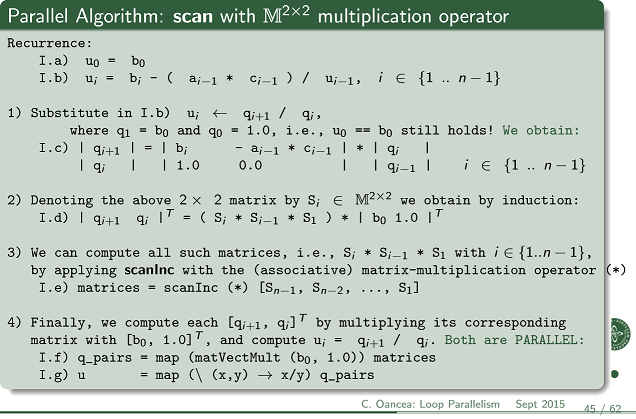
\includegraphics{images/parallelizing}
\end{figure}
\subsubsection{The Work}
In addition to the \texttt{scanInc} implementation, we also made several optimizations. Many of the changes are minor, and include re-using shared memory. Both \texttt{u} and \texttt{uu} have been moved to shared memory.

Whenever there were consecutive \texttt{+=} operations in \texttt{explicitX} and \texttt{explicitY}, we created a local variable to hold the value until the final \texttt{+=} operation.

The following changes are performed in order to achieve memory coalesced access in our CUDA kernels:
\begin{description}
\item[explicitX] is changed to compute the transpose of \texttt{u}.
\item[explicitY] writes directly to the transpose of \texttt{u}.
\item[implicitX] computes the transpose of \texttt{a}, \texttt{b}, and \texttt{c}.
\item[tridag] is called on \texttt{u}, \texttt{a}, \texttt{b}, and \texttt{c}, and thus these four arrays are transposed before calling the first \texttt{tridag}.
\item[implicitY] needs to use the transpose of \texttt{u}. \texttt{Tridag} however wrote to \texttt{u}, and thus we must transpose the new value of \texttt{u}.
\end{description}

\subsubsection{Correctness}
Several variables are moved to shared memory, some of the kernels are computed transposed, and some use transposed inputs as compared to the original: \texttt{explicitX} calculates \texttt{u} transposed; \texttt{explicitY} accumulates values into \texttt{u} transposed; \texttt{implicitX} calculates transposed \texttt{a}, \texttt{b}, and \texttt{c}, followed by transposing the results (so that we receive standard \texttt{a}, \texttt{b}, and \texttt{c}); \texttt{implicitY} uses the transposed \texttt{u} (\texttt{u} is modified by the first \texttt{tridag} call before \texttt{implicitY} is calculated), so \texttt{u} is transposed just before \texttt{implicitY} is called.

We are assured of the correctness of these modifications. We know that the variables we moved to shared memory were not going to cause race conditions, since they are accessed as read variables. The transposed/regular variables do not matter as long as the calculations work the same, and for some of the operations it is easier to perform them with a transposed version of the matrices.
\section{Results}
Table \ref{fig:results} shows the total execution times for the four versions of the code: Sequential CPU, OpenMP CPU, Na\"ive CUDA, and Optimized CUDA for both the small and large dataset. We have deliberately excluded the medium dataset since the \texttt{tridag} CUDA kernel only runs on datasets matching the dimensions of the CUDA kernel.
\subsection{Comparisons}
\begin{table}[h]
\centering
\begin{tabular}{l r r}
\toprule
\multirow{2}{*}{Version}        & \multicolumn{2}{c}{Total execution time (microseconds)} \\
                    & Small     & Large \\
\midrule
Sequential CPU      & 2297659   & 216305907 \\
OpenMP CPU          & 213948    & 10132446  \\
Na\"ive CUDA        & 92787     & 6975193   \\
Optimized CUDA      & 60867     & 3647836   \\
\bottomrule
\end{tabular}
\caption{\label{fig:results} Results of the three different implementations.}
\end{table}
\subsection{Conclusion}
\bibliographystyle{plain}
\bibliography{bibliography}
\end{document}          
